\chapter{Numerical results} \label{sec:num_results}
In order to quantify the results of the previous chapter, it is usefull to parameterize the solutions of the rate equations above, especially the solution for the $B-L$ asymmetry described by \eqref{eq:B-L_rate_expanding_interaction} or \eqref{eq:B-L_rate_expanding_interaction_rel} using the so called final efficiency factor $\kappa_f$ defined via
\begin{equation}
\lim\limits_{z\rightarrow\infty}\frac{n_{B-L}}{n_\gamma^{eq}}=\frac{3}{4}\epsilon\kappa_f,
\label{eq:final_efficiency}
\end{equation}
with $n_\gamma^{eq}=2\zeta(3)T^3/\pi^2$ the equilibrium density of photons and $\epsilon$ the CP-asymmetry parameter. It is now more convenient to rewrite the rate equations in terms of
\begin{equation}
	X_i\equiv\frac{n_i}{T^3},
	\label{eq:X_i}
\end{equation}
 with $i=B-L,N$. Using this substitution, one has to consider the transformation \cite[Eq. 7.1]{Wormann:2016yyi}
\begin{equation}
\frac{d}{dt}(X_iT^3)+3Hn_i=\frac{dX_i}{dt}T^3.
\end{equation}
Also, since the limit in \eqref{eq:final_efficiency} considers $z$ instead of the time $t$ one has to change the dependence from $t$ to $z$ by using
\begin{equation}
\frac{d}{dt}=\frac{dz}{dt}\frac{d}{dz}=\frac{dz}{dT}\frac{dT}{dt}\frac{d}{dz}=-\frac{M_N}{T^2}(-HT)\frac{d}{dz}=zH\frac{d}{dz},
\end{equation}
where the relation $dT/dt=-HT$ \cite[p. 3]{HahnWoernle:2009qn} was used. \newline\indent
Combining all these results in the new, uncorrected rate equations gives
\begin{equation*}
zH\frac{dX_N}{dz}=-\Gamma_0\left(X_N-X_N^{eq}\right),
\end{equation*}
\begin{equation*}
zH\frac{dX_{B-L}}{dz}=\Gamma_0\left[\epsilon\left(X_N-X_N^{eq}\right)-\frac{3}{\pi^2}\:\left(c_\ell+\frac{c_\phi}{2}\right)z^2K_1(z)X_{B-L}\right],
\end{equation*}
Now by dividing these rate equations by the factor $zH$ and by using \eqref{eq:washout} one finally arrives at
\begin{equation}
\frac{dX_N}{dz}=-zK\left(X_N-X_N^{eq}\right),
\end{equation}
\begin{equation}
\frac{dX_{B-L}}{dz}=zK\left[\epsilon\left(X_N-X_N^{eq}\right)-\frac{3}{\pi^2}\:\left(c_\ell+\frac{c_\phi}{2}\right)z^2K_1(z)X_{B-L}\right].
\label{eq:X_B-L}
\end{equation}
To be able to relate the result of these rate equations it is useful to express equation \eqref{eq:X_B-L} in terms of
\begin{equation}
	N_{B-L}\equiv\frac{n_{B-L}}{n_\gamma^{eq}}=\frac{\pi^2}{2\zeta(3)}X_{B-L},
\end{equation}
yielding
\begin{equation}
\frac{dN_{B-L}}{dz}=\frac{\pi^2}{2\zeta(3)}\epsilon zK\left(X_N-X_N^{eq}\right)-\frac{3}{\pi^2}\:\left(c_\ell+\frac{c_\phi}{2}\right)z^3K_1(z)KN_{B-L}.
\label{eq:N_B-L}
\end{equation}
Now, in order to finally remove the last unkown parameter in \eqref{eq:N_B-L}, namely the CP-asymmetry parameter $\epsilon$ one can use the efficiency factor $\kappa(z)$, which is, analogously to \eqref{eq:final_efficiency}, defined via
\begin{equation}
	\frac{n_{B-L}}{n_\gamma^{eq}}=\frac{3}{4}\epsilon\kappa,
	\label{eq:efficiency}
\end{equation} 
where $\kappa(\infty)=\kappa_f$,to rewrite equation \eqref{eq:N_B-L} resulting in
\begin{equation}
\frac{d\kappa}{dz}=\frac{2\pi^2}{3\zeta(3)}zK\left(X_N-X_N^{eq}\right)-\frac{3}{\pi^2}\:\left(c_\ell+\frac{c_\phi}{2}\right)z^3K_1(z)K\kappa.
\label{eq:kappa}
\end{equation}
The next step will be to introduce the relativistic corrections to these rate equations. For this they have to be normalized in a similar but different way as the one in equation \eqref{eq:X_i}\cite[Eq. (7.9)]{Wormann:2016yyi}:
\begin{equation}
	X_u\equiv\frac{M_N^2}{T^5}u=\frac{z^2}{T^3}u,
	\label{eq:X_u}
\end{equation}
with $u$ given in \eqref{eq:energy_density}.\newline \indent
Substituting this for $u$ in the equations \eqref{eq:L_rate_expanding_interaction_rel}, \eqref{eq:rate_u} and \eqref{eq:B-L_rate_expanding_interaction_rel} and rewriting the rate equations according to the steps above results in\cite[p. 47]{Wormann:2016yyi}
\begin{equation}
\frac{dX_u}{dz}=-zK\left(X_u-X_u^{eq}\right),
\end{equation}
\begin{equation}
\frac{dX_N}{dz}=-zK\left(X_N-X_N^{eq}\right)+\frac{K}{z}\left(X_u-X_u^{eq}\right),
\end{equation}
\begin{equation}
\frac{d\kappa}{dz}=\frac{2\pi^2}{3\zeta(3)}zK\left[\left(X_N-X_N^{eq}\right)-\frac{1}{z^2}\left(X_u-X_u^{eq}\right)\right]-\frac{3}{\pi^2}\:\left(c_\ell+\frac{c_\phi}{2}\right)z^3K_1(z)K\kappa.
\end{equation}
The last thing needed to solve these equations are the two equlibrium distributions $X_N^{eq}$ and $X_u^{eq}$, which are given as
\begin{align}
	X_N^{eq}=\frac{1}{\pi^2}z^2K_2(z),\\
	X_u^{eq}=\frac{3}{2\pi^2}z^3K_3(z).
\end{align}
Their calculation can be looked up in appendix \ref{ap:equlibrium}.\newline \indent
Now, after everything needed to solve the rate equation is available, they were solved using the MATLAB code that can be looked up in appendix \ref{ap:matlab}. The solution starts at $z=1$, since there $p\sim M_N$ and therefore the non-relativistic expansion cannot be used for smaller $z$ \cite[p. 13]{Bodeker:2013qaa}. Also, next to $\kappa(1)=0$, two sets of initial conditions were used for $n_N$ and $u$ or $X_N$ and $X_u$ respectively, the first one being vanishing $X_N$ and $X_u$ while the second set of initial conditions are thermal ones, thermal meaning that the densities $n_N$ and $u$ start at their corresponding equilibrium values for $z=1$. Latter is the more physical and realistic scenario because for $K\gtrsim1$ a reasonable number of right-handed neutrinos will have been produced at $z=1$\cite[p. 13]{Bodeker:2013qaa}. \newline\indent
Figure \ref{fig:efficiency} shows the final efficiency factor plotted against the washout parameter $K$ with and without the relativistic corrections for vanishing und thermal initial conditions, respetively, for a temperature ranging from $10^{8}-10^{11}$GeV. It is easy to see that for small $K\lesssim$ 4 the non-relativistic approximation is not viable because for both sets of intial conditions respectively the results of the non-relativistic and the relativistic calculation differ significantly, with the greatest discrepancy appearing for vanishing initial conditions. On the other hand for $K\gtrsim$ 5 the differences between initial conditions as well as between non-relativistic and relativistic calculation disappear until the four curves run together for $K\sim$ 7. This clearly shows that for a sufficiently high washout parameter the non-relativistic approximation is a feasible way of describing the evolution of the $B-L$ asymmetry and that higher orders of relativistic corrections are not necessary to be included.
\begin{figure}[H]
	\centering
	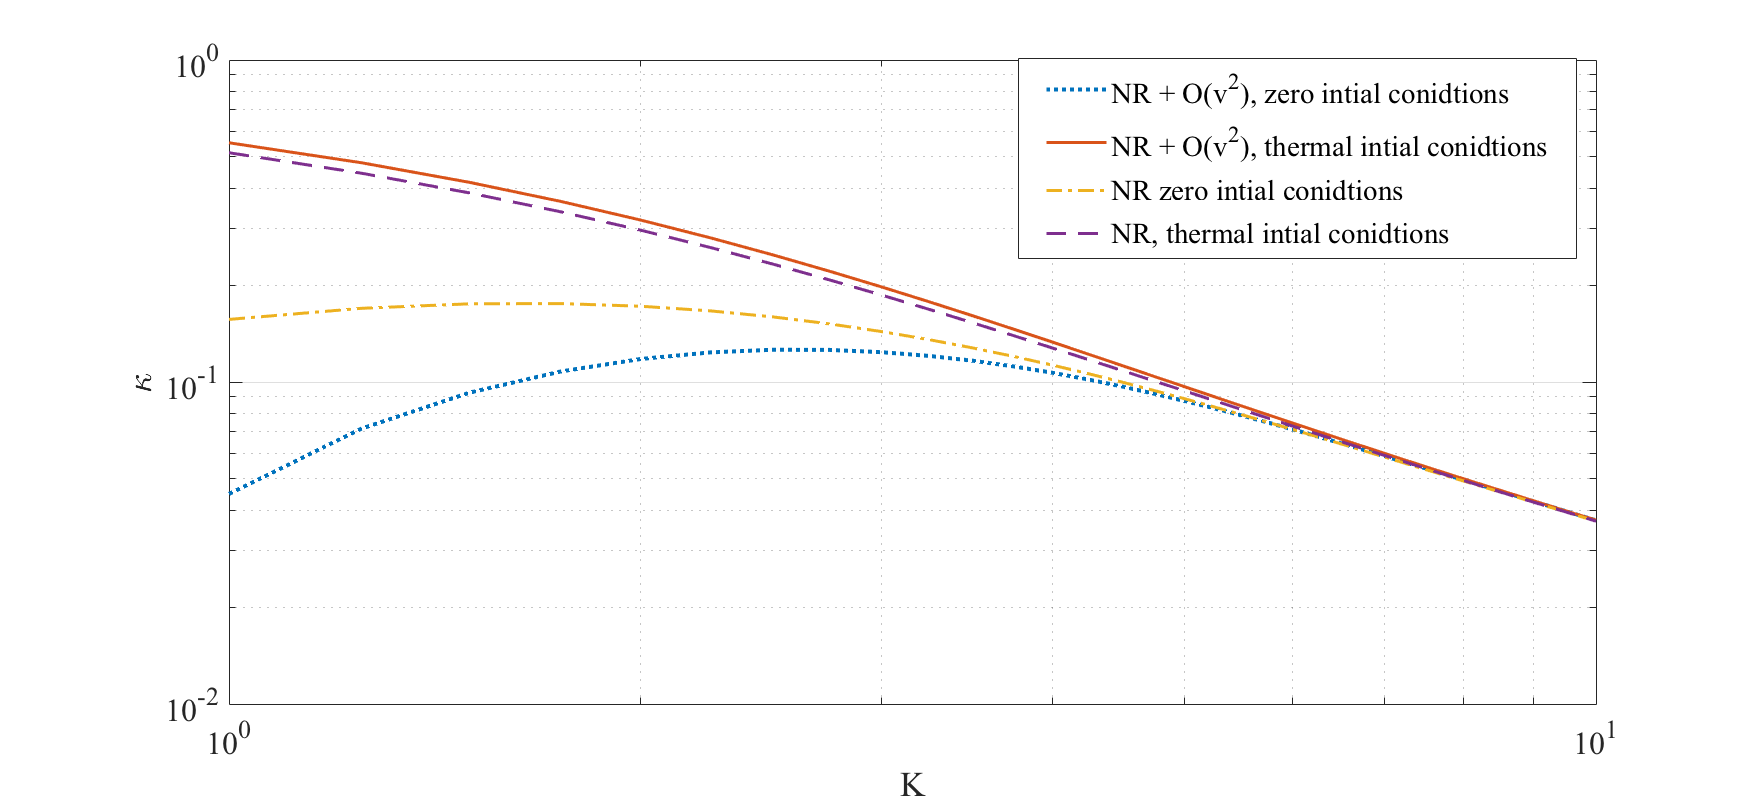
\includegraphics[width=\linewidth]{Images/efficiency}
	\caption{The final efficiency factor depending on the washout strength. The non-relativistic approximation as well as the relativistic corrections are plotted for both zero and thermal initial conditions.The temperature is in a range of $T=10^{8}-10^{11}$GeV.}
	\label{fig:efficiency}
\end{figure}
The next interesting thing to analyze is how the discrepancies between the non-relativistic approximation and the calculation containing $\mathcal{O}(p^2)$ corrrections evolve with growing $K$. This is depicted in figure \ref{fig:corrections}, where relative difference of these two results is plotted against $K$ for different temperature ranges, while thermal intial conditions were used. For small washout parameters clear differences for the different temperature ranges can be seen, however, even for the highest temperatures of $T>10^{13}$ GeV this relative difference merely surpasses 10\%. This differences then drop rapidly for every temperature until they slowly converge for $K\gtrsim10$, where the relative error is already well below 1\%. For even larger $K$, namely $K\sim20$ the relative size of the relativistic corrections is about 0.1\% for every shown temperature range. This again, clearly shows, that for a high enough washout parameter $K$ the non-relativistic approach is perfectly viable. \newline \indent
Now figure \ref{fig:corrections} can be used to analyze \ref{fig:efficiency} in more detail. As mentioned above the 4 curves in \ref{fig:efficiency} run together for $K\sim$ 7 and indeed, by looking at the green, dotted curve in \ref{fig:corrections}, the relative size of the relativistic corrections is about 1.5\% and at the endpoint of \ref{fig:efficiency} at $K=10$ it is 0.7\% and therefore the discrepancy is already below 1\%.
\begin{figure}[H]
	\centering
	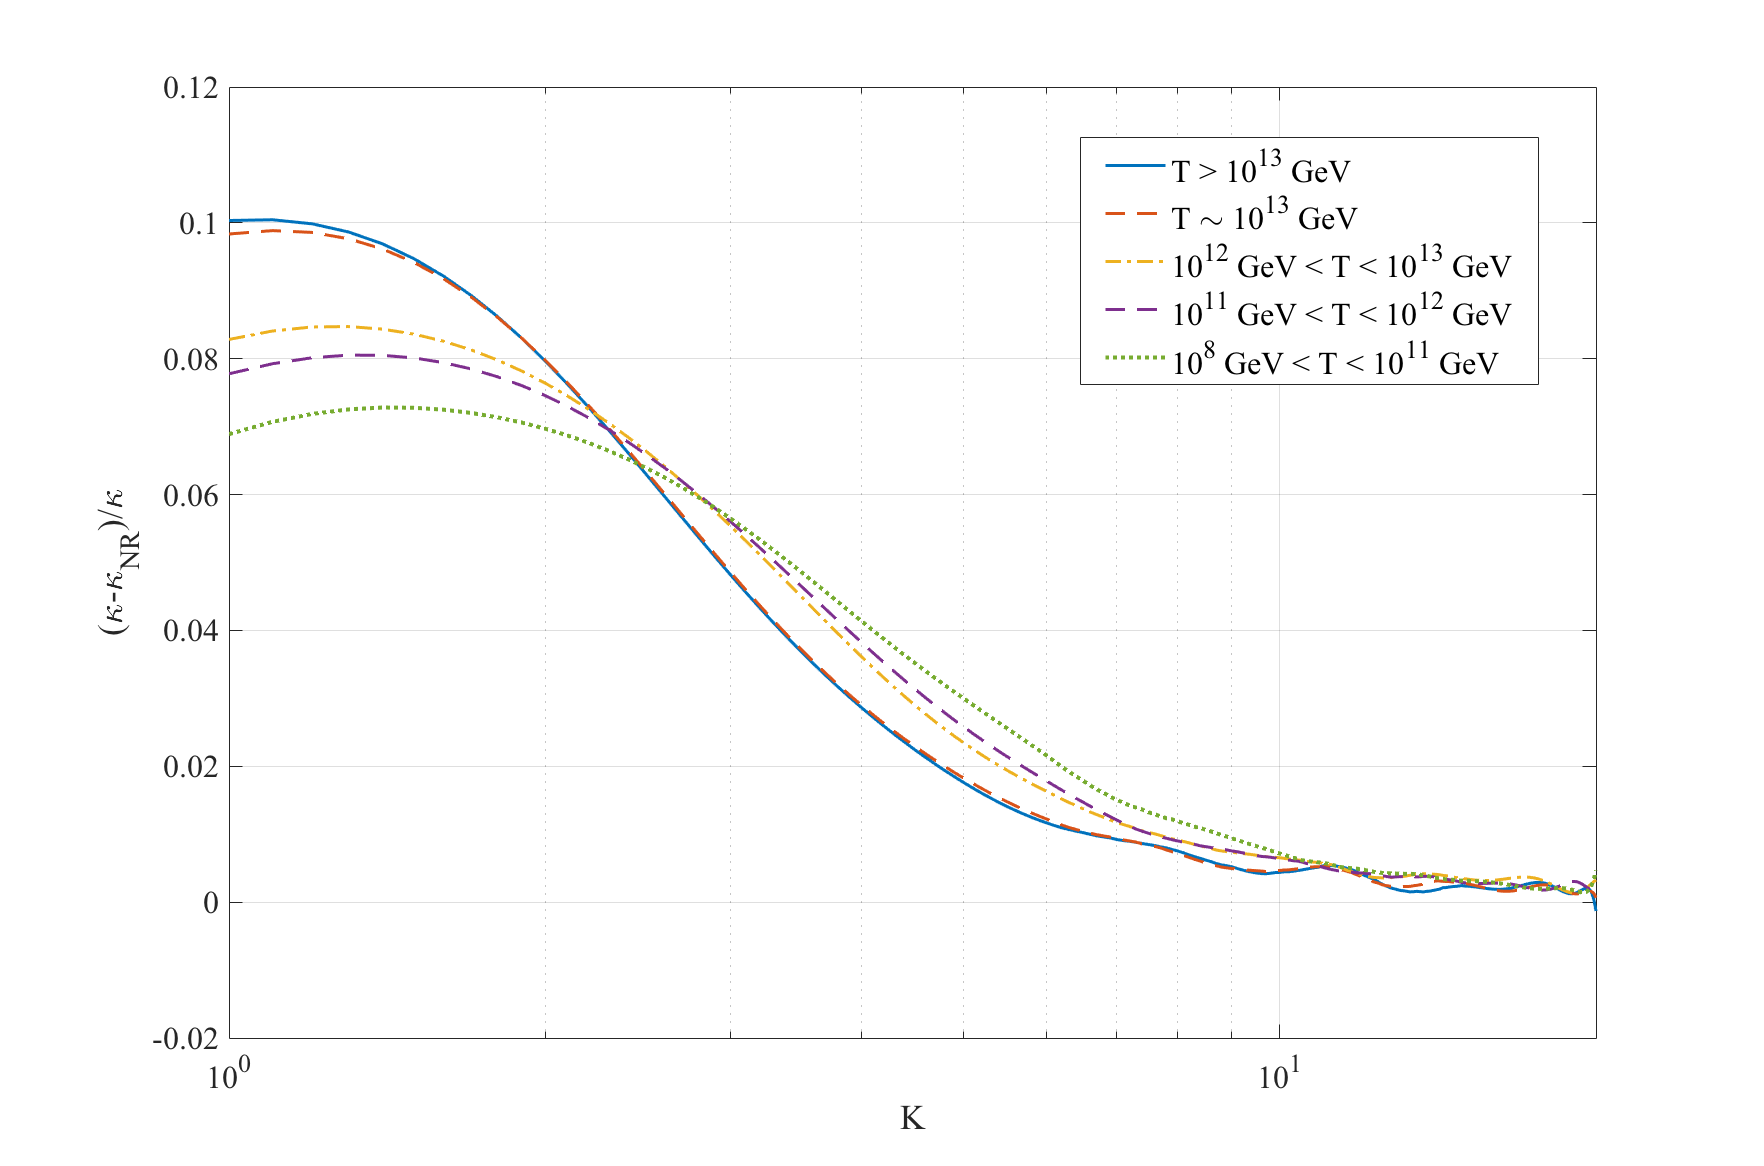
\includegraphics[width=\linewidth]{Images/corrections}
	\caption{The difference of the non-relativistic approximation and the expansion containing the relativistic corrections normalized to the relativistic solution plotted against the washout parameter for different temperature ranges, corresponding to different values of $c_\ell$ and $c_\phi$. Here thermal initial conditions were used.}
	\label{fig:corrections}
\end{figure}\noindent
Finally the effect of using the correct quantum statistics over classical Boltzmann statistics and vice versa will be studied and examined. 
During the calculations of the coefficients in the rate equations, more precisely during the calculation of $\Gamma_{B-L}$ there were two occasions in which the explicit forms of particle distributions had to be used, namely for obtaining the equations \eqref{eq:chempot_l} and \eqref{eq:chempot_phi} and even before that for calculating the product $f_\ell f_\phi$. \newline \indent
In the first case quantum statistics were used for leptons and Higgses respectively, yielding the result given in that section. If one uses classical Boltzmann statistics the result changes by a seemingly not that impactful numerical coefficient of 12/$\pi^2$, yielding
\begin{equation}
\Gamma_{B-L}=\frac{1}{4}\:\left(c_\ell+\frac{c_\phi}{2}\right)z^2K_1(z)\Gamma_0,
\label{eq:Gamma_B-l_classical}
\end{equation}
as given in appendix \ref{ap:statistics}.
\begin{figure}[H]
	\centering
	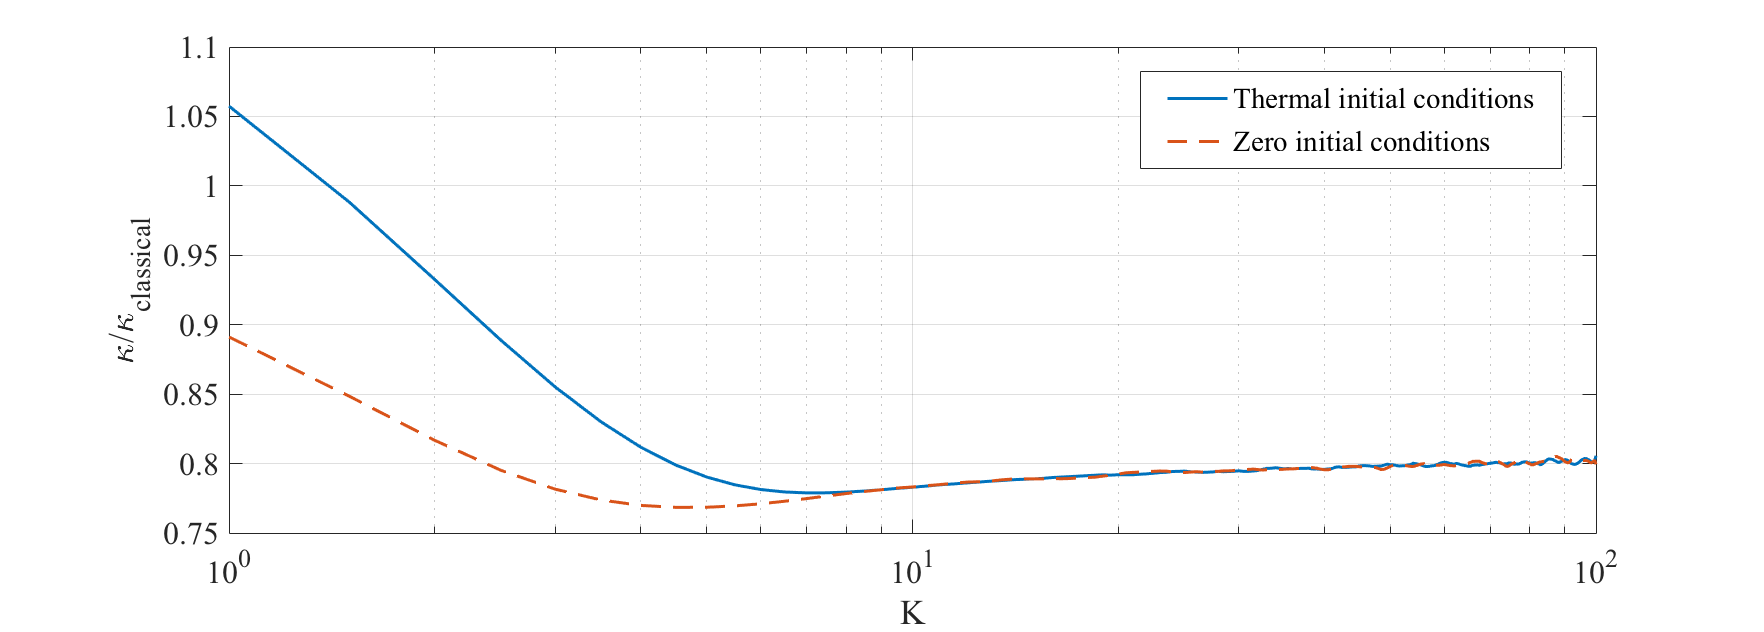
\includegraphics[width=\linewidth]{Images/quantum}
	\caption{The final efficiency factor determined using the respective quantum stastics to obtain equations for the chemical potentials of leptons and Higgses normalized by the final efficiency factor obtained by using classical Boltzmann statistics for thermal and vanishing initial conditions. $c_\ell=1$ and $c_\phi=0$ were used.}
	\label{fig:quantum}
\end{figure} \noindent
Figure \ref{fig:quantum}, however, clearly shows that using Boltzmann statistics drastically changes the final efficiency factor. For small $K$ and thermal initial conditions the classical approximation is about 5\% smaller than the result obtained using quantum statistics, while for zero initial conditions the classical approximation exceeds the quantum calculation by $\sim$11\%. For growing $K$ the classical approximation grows larger, surpassing the quantum calculation more and more and the deviation peaks at about 24\% for $K\simeq$ 5 and zero initial conditions and at about 22\% for $K\simeq$ 7 and thermal initial conditions, respectively. For an even larger washout parameter this deviation slightly lowers until it reaches around 20\% for $K\simeq$ 30 for both sets of initial conditions. From this point on $\kappa/\kappa_{classical}$ practically stays constant for growing $K$.
This clearly highlights the importance of using the right statistics, as using classical statistics is a somewhat good approximation only for small washout parameters, while it completely fails for higher washout parameters.\newline \indent
On the other hand, because the Higgs particles and leptons are of high energy and the corresponding integrals do not saturate at momenta of order $T$ they can be treated using Maxwell-Boltzmann statistics, in order to calculate the quantity $f_\ell f_\phi-f_{\bar{\ell}}f_{\bar{\phi}}$. Nevertheless, it is interesting to see how using the correct quantum statistics and therefore not neglecting their quantum characteristics, affects previous results.
As also shown in appendix \ref{ap:statistics}, this leads the following correction of the coefficient $\Gamma_{B-L}$
\begin{equation}
\Gamma_{B-L}=\frac{3}{\pi^2}\:z^3\left(\frac{e^{z/2}}{e^{z/2}-1}\:\frac{c_\phi}{2}+\frac{e^{z/2}}{e^{z/2}-1}c_\ell\right)\int_{1}^{\infty}dx\frac{\sqrt{x^2-1}}{e^{zx}-1}\Gamma_0.
\label{eq:B-L_corrected}
\end{equation}
\begin{figure}[H]
	\centering
	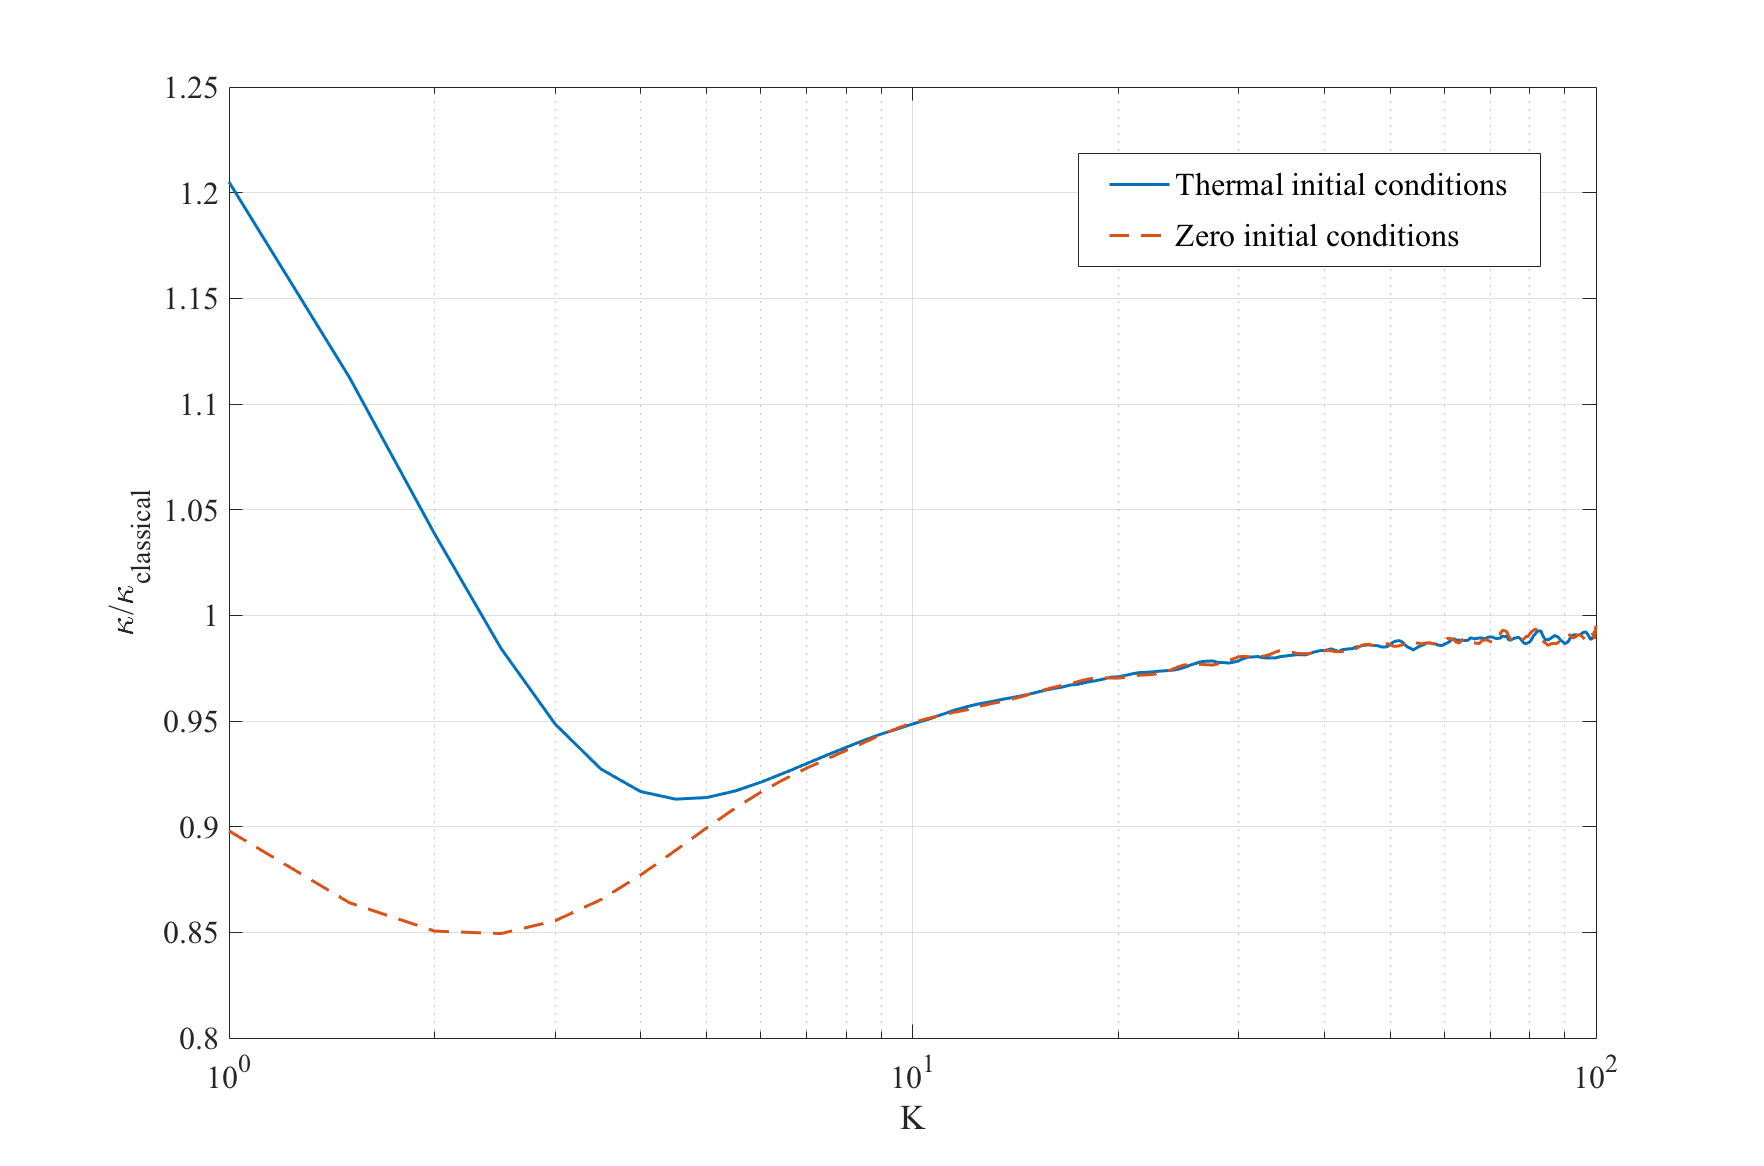
\includegraphics[width=\linewidth]{Images/quantum1}
	\caption{The final efficiency factor determined using only the respective quantum stastics for obtaining $f_\ell f_\phi$ normalized by the final efficiency factor obtained by using classical Boltzmann statistics for thermal and vanishing initial conditions. $c_\ell=1$ and $c_\phi=0$ were used.}
	\label{fig:quantum1}
\end{figure} \noindent
Figure \ref{fig:quantum1} shows how using \eqref{eq:B-L_corrected} instead of \eqref{eq:Gamma_B-l_result} affects the final efficency factor. In general the course of the graphs is similar to the ones in figure \ref{fig:quantum}, however the differences lie in the reached values of the derivation. For $K\sim$1 $\kappa_{classical}$ is about 20\% greater than $\kappa$ for thermal initial conditions and therefore the deviation here is bigger as in \ref{fig:quantum}. For zero initial conditions on the other hand the deviation of about 10\% is comparable to the one above. Now $\kappa_{classical}$ grows bigger with $K$ and surpasses $\kappa$ but the drop of $\kappa/\kappa_{classical}$ is not as severe as above, as it peaks at around 85\% for zero initial conditions and $K\sim$ 2.5, meaning $\kappa_{classical}$ is about 15\% bigger than $\kappa$. For thermal initial conditions this effect is even smaller with the discrepancy between the two efficiency factors, reaching its maximum at around 91\% for $K\simeq$ 5. For both sets of initial conditions this effect gets smaller with growing $K$, so at $K=30$, the point where a nearly constant difference of about 20\% sets in above, the difference is below 2\%. \newline \indent
This is a clear sign showing that in the latter of the cases mentioned above using a classical approximation can have a meaningfull impact on the final efficiency for a low washout parameter, but it slowly gets negligible for higher $K$ in contrast to the first case where the discrepancy between classical and quantum statistics is about 20\% even for high $K$.\newline\indent
Finally, it should be mentioned that the results shown in figure \ref{fig:efficiency}$-$\ref{fig:quantum} agree with the results depicted in Ref. \cite{Bodeker:2013qaa} and \cite{Wormann:2016yyi}.\newpage